%! Author = wolfram_e_laube
%! Date = 06.05.24

\item[(a)]
\section{Task (a): Spectrum of $x(t)$}

\subsection{Problem Statement}
The analog signal $x(t)$, defined as:
$$
x(t) = x_1(t) + x_2(t) = \sin(2\pi f_1 t) + \sin(2\pi f_2 t),
$$
with frequencies $f_1 = 4 \text{kHz}$ and $f_2 = 6 \text{kHz}$, is to be sampled with a sampling rate of $f_s = 10 \text{kHz}$. The task is to draw the spectrum of $x(t)$ before it is sampled.

\subsection{Analysis}
\subsubsection{Signal Composition}
The signal $x(t)$ comprises two sinusoidal components:
\begin{itemize}
    \item $x_1(t)$ corresponding to $\sin(2 \pi f_1 t)$ with $f_1 = 4 \text{kHz}$,
    \item $x_2(t)$ corresponding to $\sin(2 \pi f_2 t)$ with $f_2 = 6 \text{kHz}$.
\end{itemize}
In the frequency domain, each sine wave component is represented by delta functions at both its frequency and its negative counterpart, resulting in spikes at $\pm 4000 \text{Hz}$ and $\pm 6000 \text{Hz}$.

\subsubsection{Frequency Domain Representation}
The spectrum of $x(t)$ will therefore feature delta spikes at the frequencies corresponding to the components of the signal.
This is due to the representation of sinusoids in the frequency domain, which are depicted as:
$$
\sin(\omega t) = \frac{e^{i\omega t} - e^{-i\omega t}}{2i}
$$

\subsection{Conclusion}
The spectrum of $x(t)$ distinctly displays delta spikes at the frequencies of the sinusoidal components,
clearly indicating their presence at $\pm 4000 \text{Hz}$ and $\pm 6000 \text{Hz}$.
This visualization is crucial for understanding the frequency content of the analog signal before considering the effects of sampling,
such as aliasing or frequency folding.
Understanding this spectrum is foundational for further analysis of how sampling will impact the signal in digital form.

\begin{figure}[h]
    \centering
    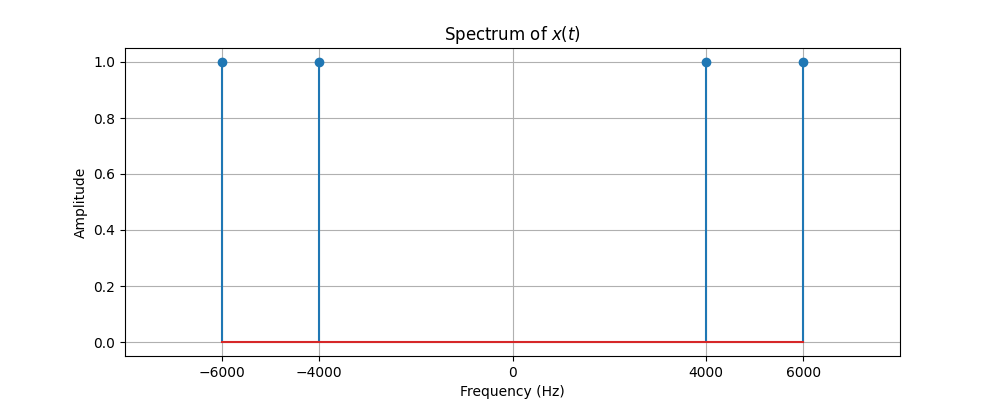
\includegraphics[width=0.49\textwidth]{fig/ex1_a_plot}
    \caption{Spectrum of \(x(t)\)}
    \label{fig:ex1_a_plot}
\end{figure}
